\chapter{Related Work}
\label{chp:relatedwork} 


\section{Social Network Services}
\paragraph{}
A social network service (SNS), is a platform used to establish social networks of different people. These people often share a common interest or activity \cite{SNS}. 
\paragraph{}
Online social networks (OSNs) is a large part of the social network services. From online social networks was first introduced until today, the popularity and complexity has grown drastically, with a hundreds of millions active users \cite{OSN}. OSNs have a peer-to-peer architecture, and therefore makes it easy for members to initiate communication with whom they want, given that they are also connected to the network. OSNs also enables the possibility for people to easily publish and retrieve information about subjects of interest \cite{DPBook}. 

The internet has caused the creation of several information sharing systems. Among these systems are the Web and OSNs. As mentioned before, the popularity of OSNs has grown drastically, and have become among the most popular sites on the Web. With this change, there has also been a change in what is centralized and in focus. The Web is to a large extent organized around content, while OSNs on the other hand are organized around users. This change has lead to the importance of understanding user behaviour. A user is often represented with a profile on OSNs. To obtain a profile the user, in most cases, must register the site. When a user is given a profile, it is normal for the user to provide information about themselves. This information could for example be date of birth, home town, sex, name (or pseudonym) and maybe a profile picture. The social network is formed when users start connecting with each other. The reason for these connections are numerous; real-life friends, real-life acquaintances, colleagues, share an interest/activity or if you are interested in the information contributed by the other user \cite{OSNpaper}. 

\paragraph{}
Since Facebook was introduced to the public in 2006, it has grown to be the largest online social network (OSN) in the world. The growth of Facebook has made it necessary to introduce new ways to manage privacy and ensure a secure online environment. The privacy embedded in the program/app etc. is not enough to ensure such an environment, due to the interdependent privacy issues. Your privacy is to a large extent affected by the privacy decision of others. We will elaborate these privacy issues later in our report. 


\section{Interdependent Privacy}

\section{The History of Facebook}
When Mark Zuckerberg enrolled at Harvard in 2002, he had decided to major in psychology  “I just think people are the most interesting thing—other people,” he said. “What it comes down to, for me, is that people want to do what will make them happy, but in order to understand that they really have to understand their world and what is going on around them” \cite{MeMedia}. He showed an interrest and passion to connect people together and crate Harvard more open. 

\begin{figure}[h!]
\centering

\includegraphics[width=0.2\textwidth]{facebook-icon.png}
\caption{The Facebook Icon}
\end{figure}

\paragraph{}
It all started in October 2003 when the Harvard sophomore Mark Zuckerberg and three of his classmates created the web page facesmash. Zuckerberg hacked into the administrative database to extract the ID photos of all the students of the different houses. The web page presented two and two photos creating a “hot or not” game for his fellow students. The votes were counted and created a top-ten list of the cutest poeple in each house. Within the first hour facesmash had 450 visitors and 22 000 photo-views. After numerous complaints from professors and fellow students, Harvard administration shut down Zuckerbergs Internet connection after a few days. Harvard charged Zuckerberg for violating individual privacy, violating privacy and breach of security for stealing the photos. Zuckerberg agreed to take the web page down and got away with just a warning.

\paragraph{}
After facesmash Zuckerburg was known around campus as a programming prodigy. Harvard seniors Tyler and Cameron Winklevoss and Divya Narendra had since 2002 been working on a social networking page - HarvardConnection, where students could create a profile, and though that share some personal information and post pictures and share this with large and small communities that one could be part off. They wanted Zuckerbergs help to finalize their project so that the page could be up and running before they graduated. Zuckerberg agreed to help at the same time as presuing his own projects. Harvard offers a class directory to all freshman's, this directory is also known as the "facebook". This "facebook" contains a picture of all the students, name, date of birth, home town and high school. This so that the freshman's could get to know each other. Harvard's plan was to eventually get this online. Since Harvard had not gotten to it yet,  Zuckerburg decided to to the job himself. He wanted to create a page where people signed up and created their own profiles, and in that way could post some personal information about themselves, and have control over what was posted. After ten days of intensive work Zuckerberg almost finished the cite. The cite was kept simple and intuitive, and everybody with a Harvard e-mail address could create a profile. The profile consisted of a profile picture, name and some personal information such as taste in books, music, films and favourite quotes. Users could link to their friend's profiles and by using a "poke" button let others know that you have visited their profile. Thefacebook went public February 4, 2004, and to get the word spread they sent it out on the Kirkland house mailing list, that contained over 300 students. it did not take long until the other houses heard and within twenty-four hours close to fifteen hundred people ha registered. “I think it’s kind of silly that it would take the university a couple of years to get around to it,” he said. “I can do it better than they can, and I can do it in a week.” \cite{MeMedia}. Later the same year the three founders of HarvardConnection -now called ConnectU, files a lawsuit against Zuckerburg. Stating that he broke their oral contract, stole their idea, and delayed working on their site to be able to finish his own site, Thefacebook, first. Zuckerburg denied doing anything wrong, and stated that he had proof that he did not steal the idea from the HarvardConnection. Just a few months later Facebook filed a countersuit. Facebook accused ConnectU with defamation. The case have been going on for years. In 2011 the Winklevoss brothers dropped the lawsuit and accepted a $ 65 $ million settlement \cite{droppLawsuit}.

\paragraph{}
There was already similar pages out there, like Friendster and myspace.com. Especially on myspace.com people played roles, giving themselves out to be someone else. Teenage girls pretending to be older and grown men giving themselves out to be young girls. There is nowhere to validate that the person really is who they give themselves out to be. This limits to what extent people posts personal information. With Thefacebook.com you have to sign up with a valid Harvard e-mail address, in that way you know that they are actual people, and mostly students. This made it easier to post more personal information like cell-phone number, home address and even sexual orientation. The concern was not about security but more about wasting time, it became and addictive pleasure. 

\paragraph{}
It didn't take long before Mark Zuckerberg began to receive e-mails from other colleges, requesting to get Thefacebook at their schools. The site was easily scalable, the concern rather laid in how to maintain the intimacy and the clubby appeal. When Thefacebook expanded to Colombia, Yale and Stanford, students were only able to search and see people from their respective college. Only with permission from a student from an other college could you add the person to your friend list. This is a key factor to Facebook's success. Zuckerberg wanted people to post personal information and create a more open school community.

\paragraph{}
In June 2004, when the school year was over, Thefacebook had expanded to over forty schools, with a 150 000 users. With the rapid expansion, the need for investors and more capacity increased. Zuckerburg moved his base to California and removed the "the" from the name. Thefacebook became just Facebook.

October 2005 Facebook expanded to universities in England, Mexico and Puerto Rico, and in September 2005 a high school version was available \cite{FacebookHistory}. This was a big step for Facebook. All high school members need an invitation to be able to join.  Zuckerburg launched the possibility for all users to see the profiles and send friend request to everyone in the network, the older uses had strong objections. College students did not like the idea of high school kids looking at their profiles and being able to befriend them. But with the rapid expansion Facebook was forced to make the site more open and knock down some of the walls dividing the users. Facebook made it possible for employees at different companies like apple and Microsoft could join the network. 
At the end of 2005 Facebook was used at over 2000 colleges and at over 25 000 high schools in United states, Canada, Mexico, England, Australia, New Zealand and Ireland. 

Up to this point you had to be a student at a college of High school, or employee at a certain company to be able to join the network. After September 2006 everyone over the age of thirteen, with an valid e-mail address, could join. The site was no longer restricted to schools and was now open to the whole world. 


\section{Amazon Mechanical Turk}
\paragraph{}
The growth of the Internet have made it easier to conduct studies, surveys and so on. One commonly used technique for conducting these studies and surveys are called \emph{crowdsourcing}. Crowdsourcing is a technique where you outsource a job to a undefined group of people. The beneficial aspects with crowdsourcing is that you are provided access to a large set of people who are willing to do the tasks you want done, for low pay \cite{AMT}.

\paragraph{}
Amazon Mechanical Turk is a good example of a crowdsourcing site. Amazon Mechanical Turk is a Internet marketplace where human intelligence is utilized to perform various tasks \cite{amazonweb}. The people using Mechanical Turk are separated into two groups. You have the \emph{requesters} that post jobs/tasks, and the \emph{workers} who can choose from these jobs/tasks, and execute them for pay \cite{AMT}. 

\paragraph{The Turk}
The name "Mechanical Turk" comes from a chess-playing automaton from the  late 18th century. The Turk, as it was called, was a construction made to seem like a automatic chess-playing machine. In reality there was a chess-pro inside the machine, that steered the arms of the doll that was on the other side of the chess-board. The Turk was constructed in 1770 by the Austro-Hungarian Wolfgang von Kempelen. The reason for this construction was that von Kempelen wanted to impress the Empress Maria Theresia of Austria. 
The Turk toured around Europe and in America for decades, without anyone knowing the secret of the machine. The chess-pro that operated the construction played and defeated many, including Benjamin Franklin and Napoleon Bonaparte. Although many suspected that the Turk was steered by a 
hidden human, the trick was not exposed before 1820. The Turk was ruined in a fire in 1854 \cite{theturk}.

\begin{figure}[h!]
\centering
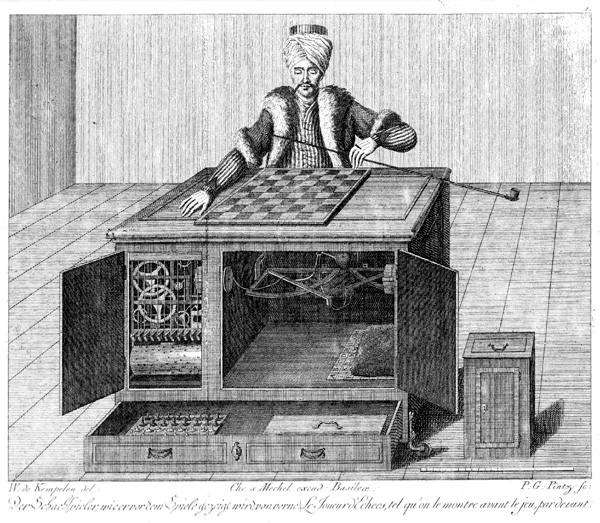
\includegraphics[width=0.7\textwidth]{Turk-open.jpg}
\caption{Engraving of the Turk. This shows the Turk with open doors and the different parts inside of the Turk. Wolfgang von Kempelen may have drawn this picture himself, since he was a talented engraver \cite{theturk}.}
\end{figure}

\paragraph{Advantages with Amazon Mechanical Turk}
There are several advantages of using AMT for conducting behavioural research surveys. Amazon Mechanical Turk enables the opportunity to reach out to a wide audience, since it provides access to a large subject pool \cite{AMT}. When conducting a survey or other research for example in connection with school projects etc., you seldom have access to a large subject pool. Usually you may get your friends to contribute, and maybe some other people going to the same school or a few people living in the same place. The results of this survey or research will most likely be reflected by lack of diversity. If you use Amazon Mechanical Turk instead, you get yet another advantage; subject pool diversity. The workers on Mechanical Turk are spread all over the world, and have different backgrounds. They have different religions, ethnicity, languages, different positions in society (economical), and age. The one last advantage with Mechanical Turk worth mentioning is that you get access to all the aspects mentioned above at a low cost. The workers are willing to take jobs and perform task for relatively low pay. Research done by Horton and Chilton \cite{amtpay} shows that the least amount of pay a worker is willing to accept for a task is \$1.38, and they call this amount \emph{reservation wage}. 




